\subsection{Modultest af optagesystemet}
I optagesystemet testes først modulerne hver for sig. 
Derefter laves der løbende integrationstests. 
\subsubsection{Timer}
Lydmodulet er testet vha. debugging med Atmel-ICE i projektet \textit{mic\_FHT\_test}.
Først er samplefrekvensen verificeret vha. et oscilloskop på ben 12 (PORTB6). 
På figur \ref{fig:test_fs} ses det, at frekvensen er $20 kHz$.

\begin{figure}[H]
	\center
	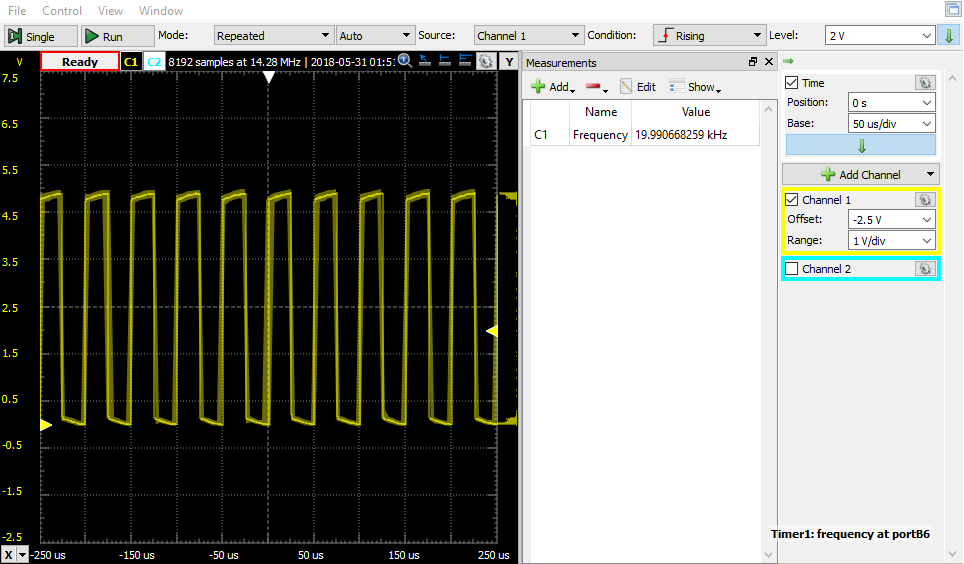
\includegraphics[width=0.8\textwidth]{Figur/test_timer_freq.png}
	\caption{Samplefrekvens fra Timer 1}
	\label{fig:test_fs}
\end{figure} 

\subsubsection{ADC}
Derefter testes ADC'en med et signal fra tonegenerator på Analog Discovery. Signalet læses ud ved første breakpoint, og plottes i Excel, som set til venstre på figur \ref{fig:1kHz_plot}. 
Det ses, at plottet ligner en sinuskurve, og at amplituden på $2 Vpp$ næsten når rails på ADC'en.

\begin{figure}[H] 
	\begin{center}
		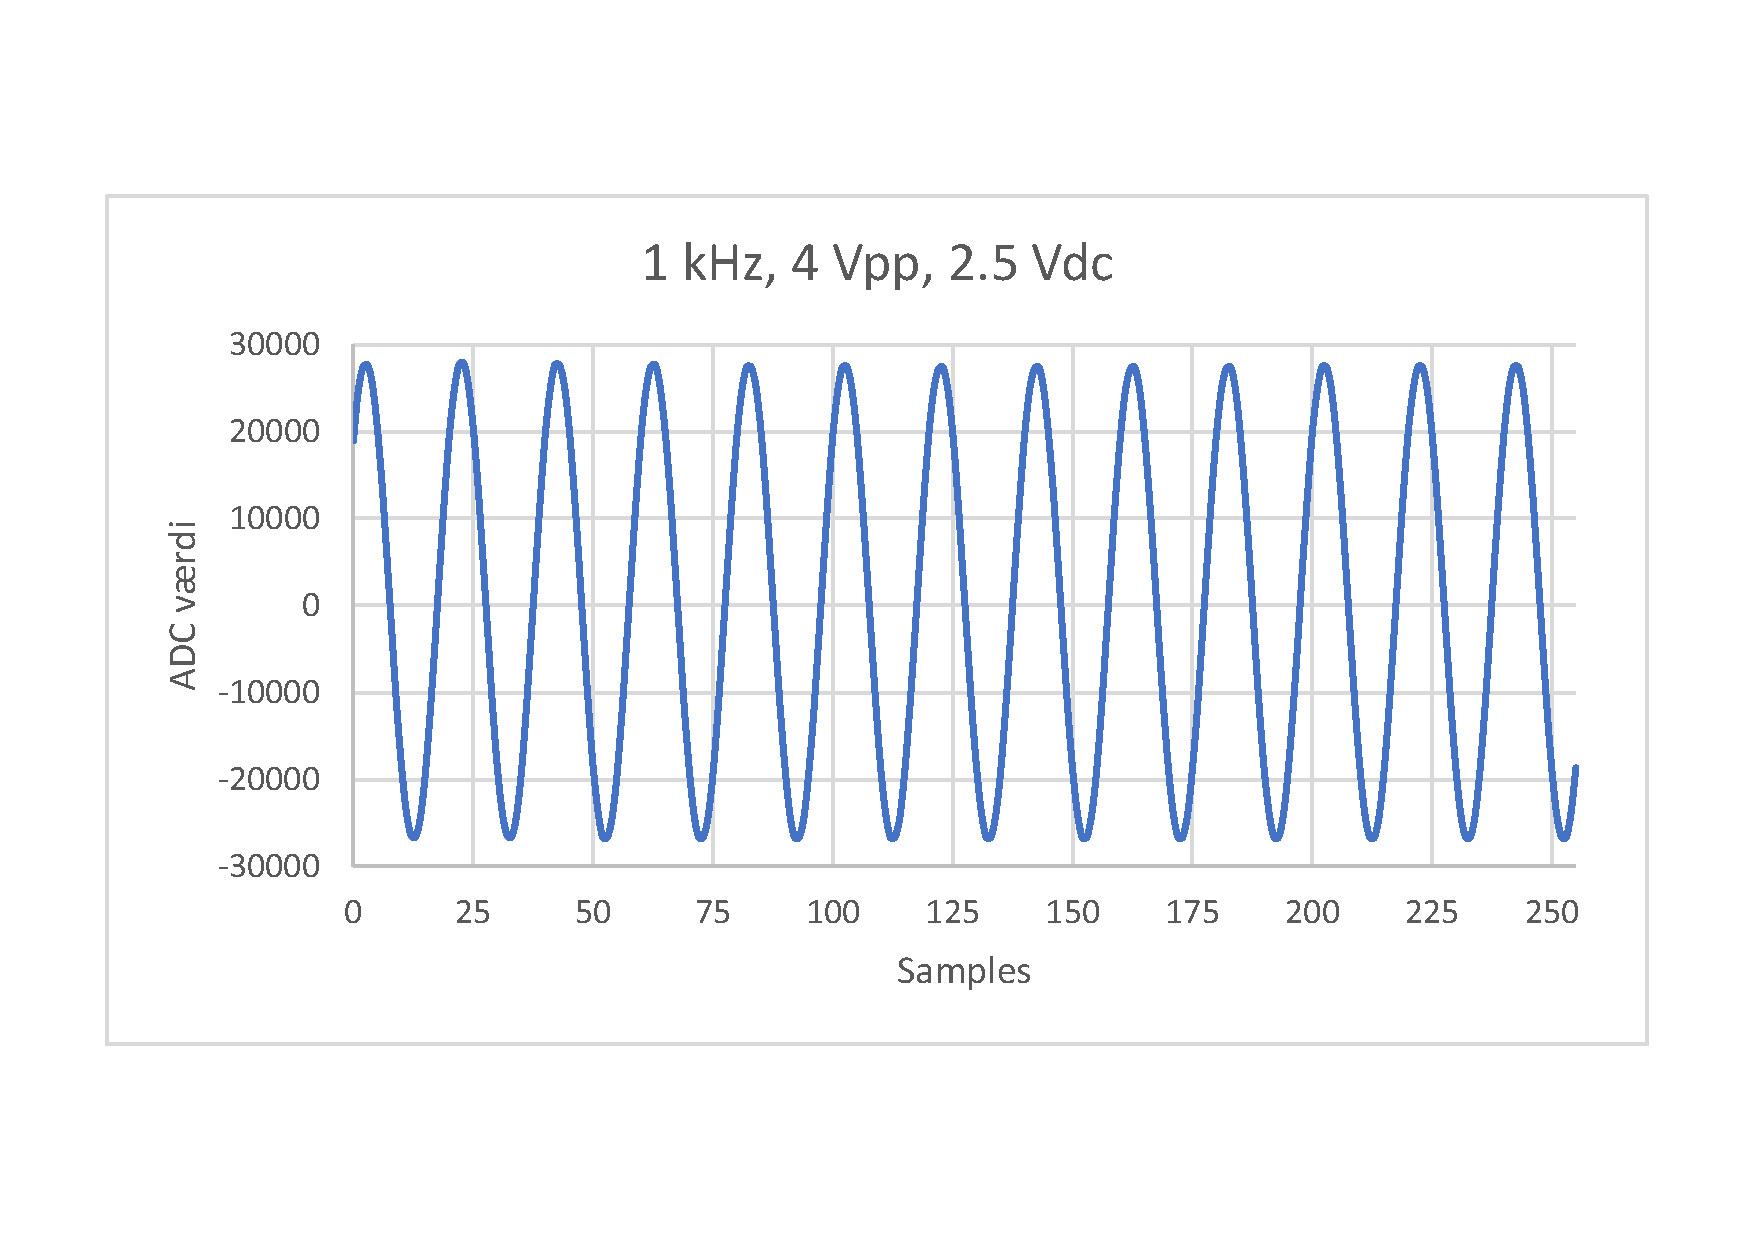
\includegraphics[width=.45\linewidth, trim={0, 2.5cm, 1.8cm, 0}, clip]{Figur/1kHz_time_plot.pdf}\quad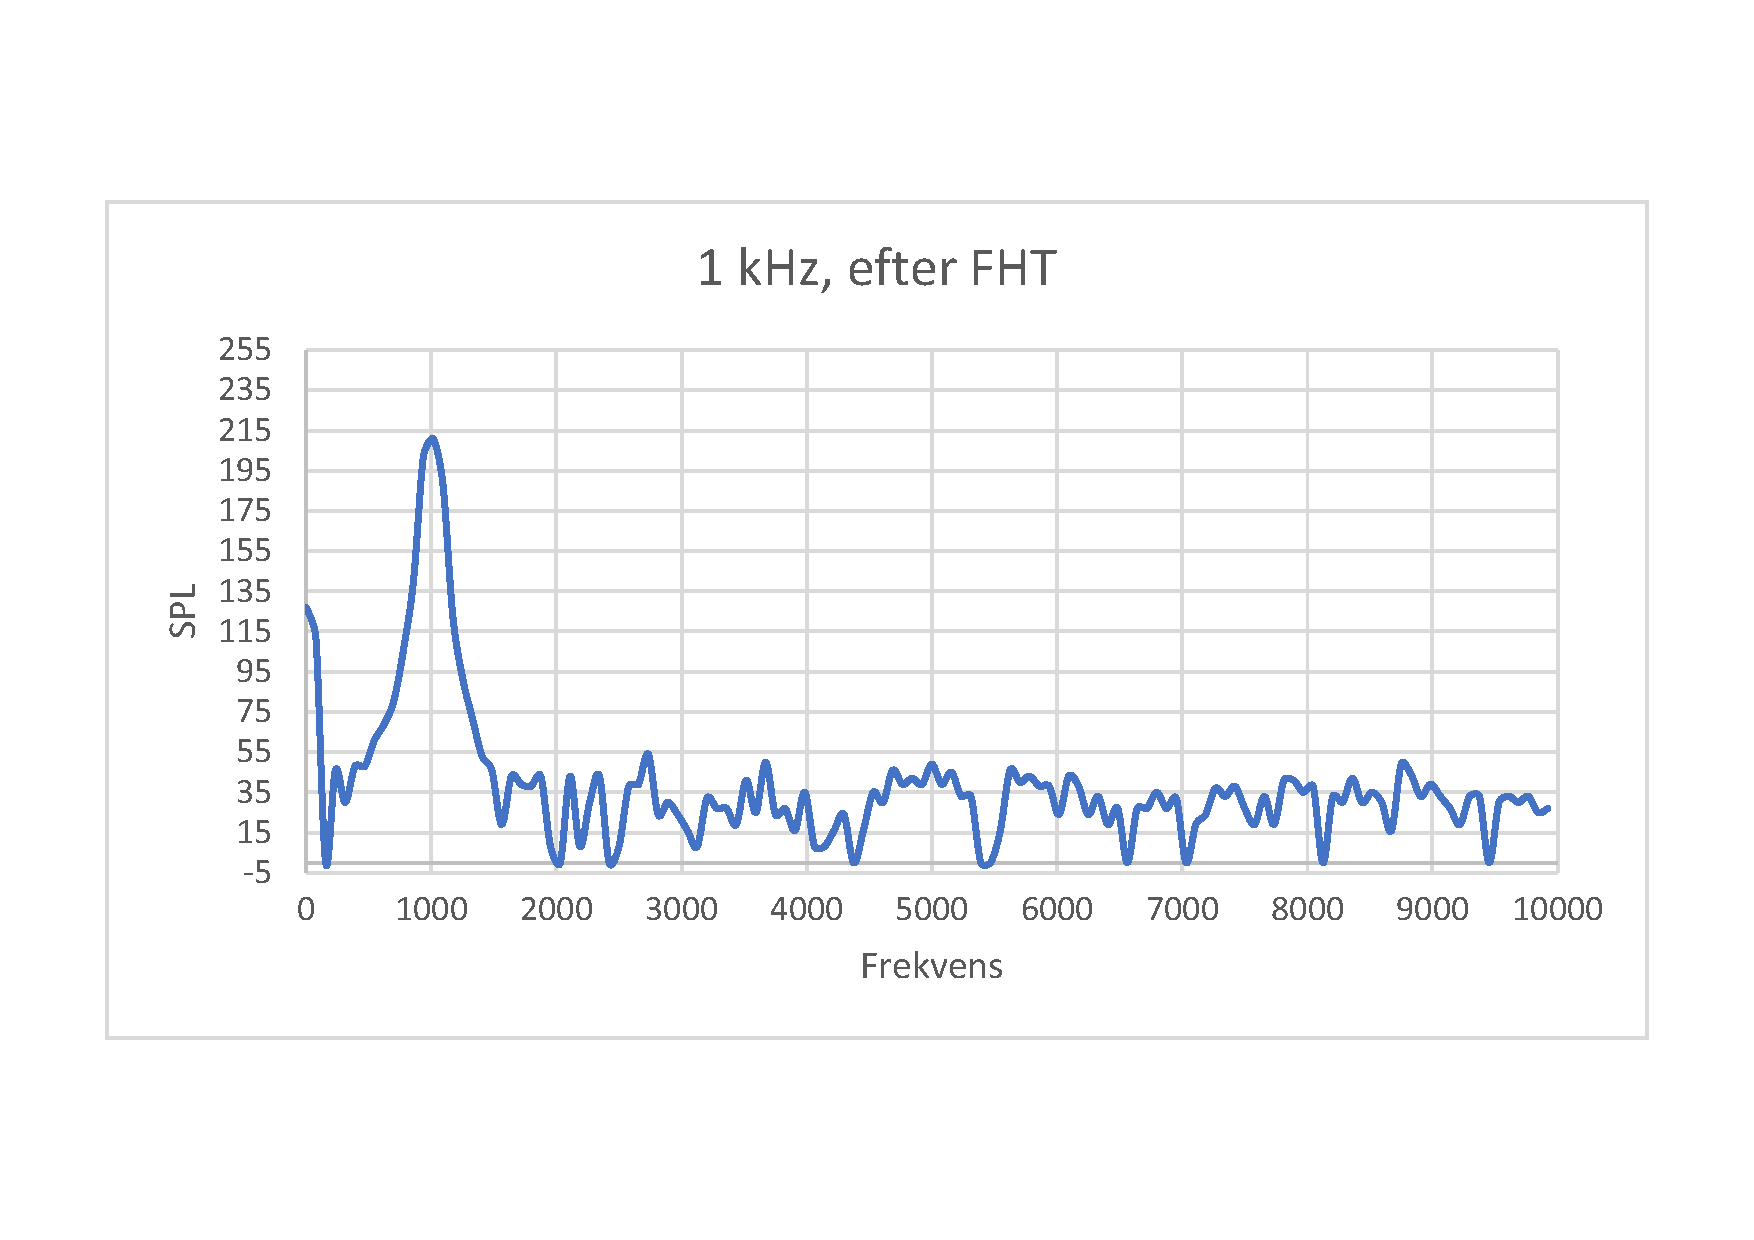
\includegraphics[width=.45\linewidth, trim={1.8cm, 2.5cm, 0, 0}, clip]{Figur/1kHz_FHT_plot.pdf}\quad
		\caption{1 kHz fra funktionsgenerator i tid- og frekvensdomænet }
		\label{fig:1kHz_plot}
	\end{center}
\end{figure}

\subsubsection{FHT}
Der singlesteppes ned til behandlingen er gennemført, og outputtet ses plottet til højre på figur \ref{fig:1kHz_plot}. 
På figuren ses tydeligt en stor peak ved $1 kHz$, altså virker FHT algoritmet. 
Resultatet understøttes også af variablen $freq$, der viser, at den kraftigste frekvens i spektret er $1016 Hz$. 
SPL-værdien kan ikke bruges, da den ikke er kalibreret, og der i øvrigt ikke er tale om et faktisk lydtryk. 

\subsubsection{Anti-aliaseringsfilter}
Efter softwaren er verificeret, kan samspillet med hardware testes. 
Først testes anti-aliaseringsfilterets lavpaskarakter, vha. en netwærksanalyse på Analog Discovery.
Bodeplottet fra den analyse ses på figur \ref{fig:LP_bodeplot}.
Det ses, at filteret er et anden ordens lavpasfilter med knækfrekvens på $10 kHz$. 
\begin{figure}[H]
	\center
	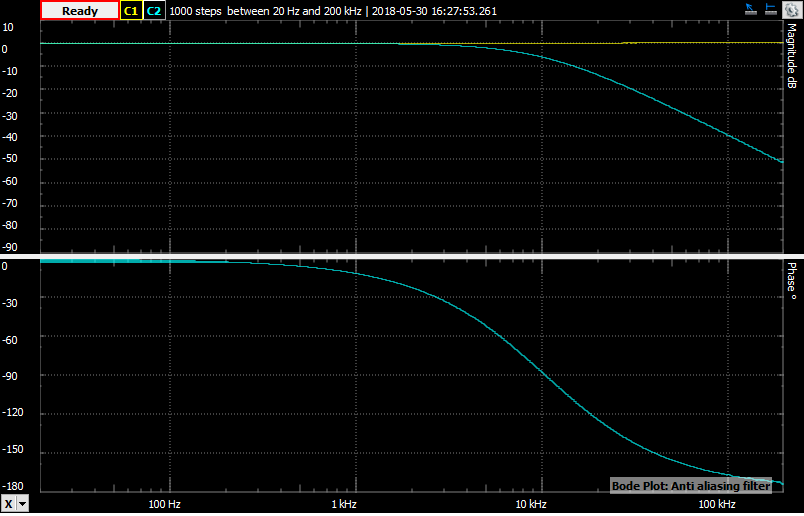
\includegraphics[width=0.8\textwidth]{Figur/test_LP_sweep.png}
	\caption{Bodeplot af anti-aliaseringsfilteret}
	\label{fig:LP_bodeplot}
\end{figure}


\subsubsection{Integrationstest med mikrofon}
Sidste skridt er at teste lydmodulet med input fra systemets mikrofon. 
Signalet læses ud som før, og plottes i både tid- og frekvensdomænet, som det ses på \ref{fig:rec_plot}.
På plottet ses det, at signalet er forvrænget til en trekantsbølge, fordi enten afspilleren eller mikrofonen går i mætning. 
Der ses tydelige harmoniske peaks op ad frekvensaksen. 
Der ses også et betydeligt bidrag af lavfrekvent støj. 
Tidsplottet viser ikke tegn på DC offset, så måske er det $50 Hz$ støj fra lysnettet, eller den blæser, som er i rummet, hvor optagelsen er lavet. 
Variablen $freq$ stemmer også denne gang overens med plottet. 

\begin{figure}[H] 
	\begin{center}
		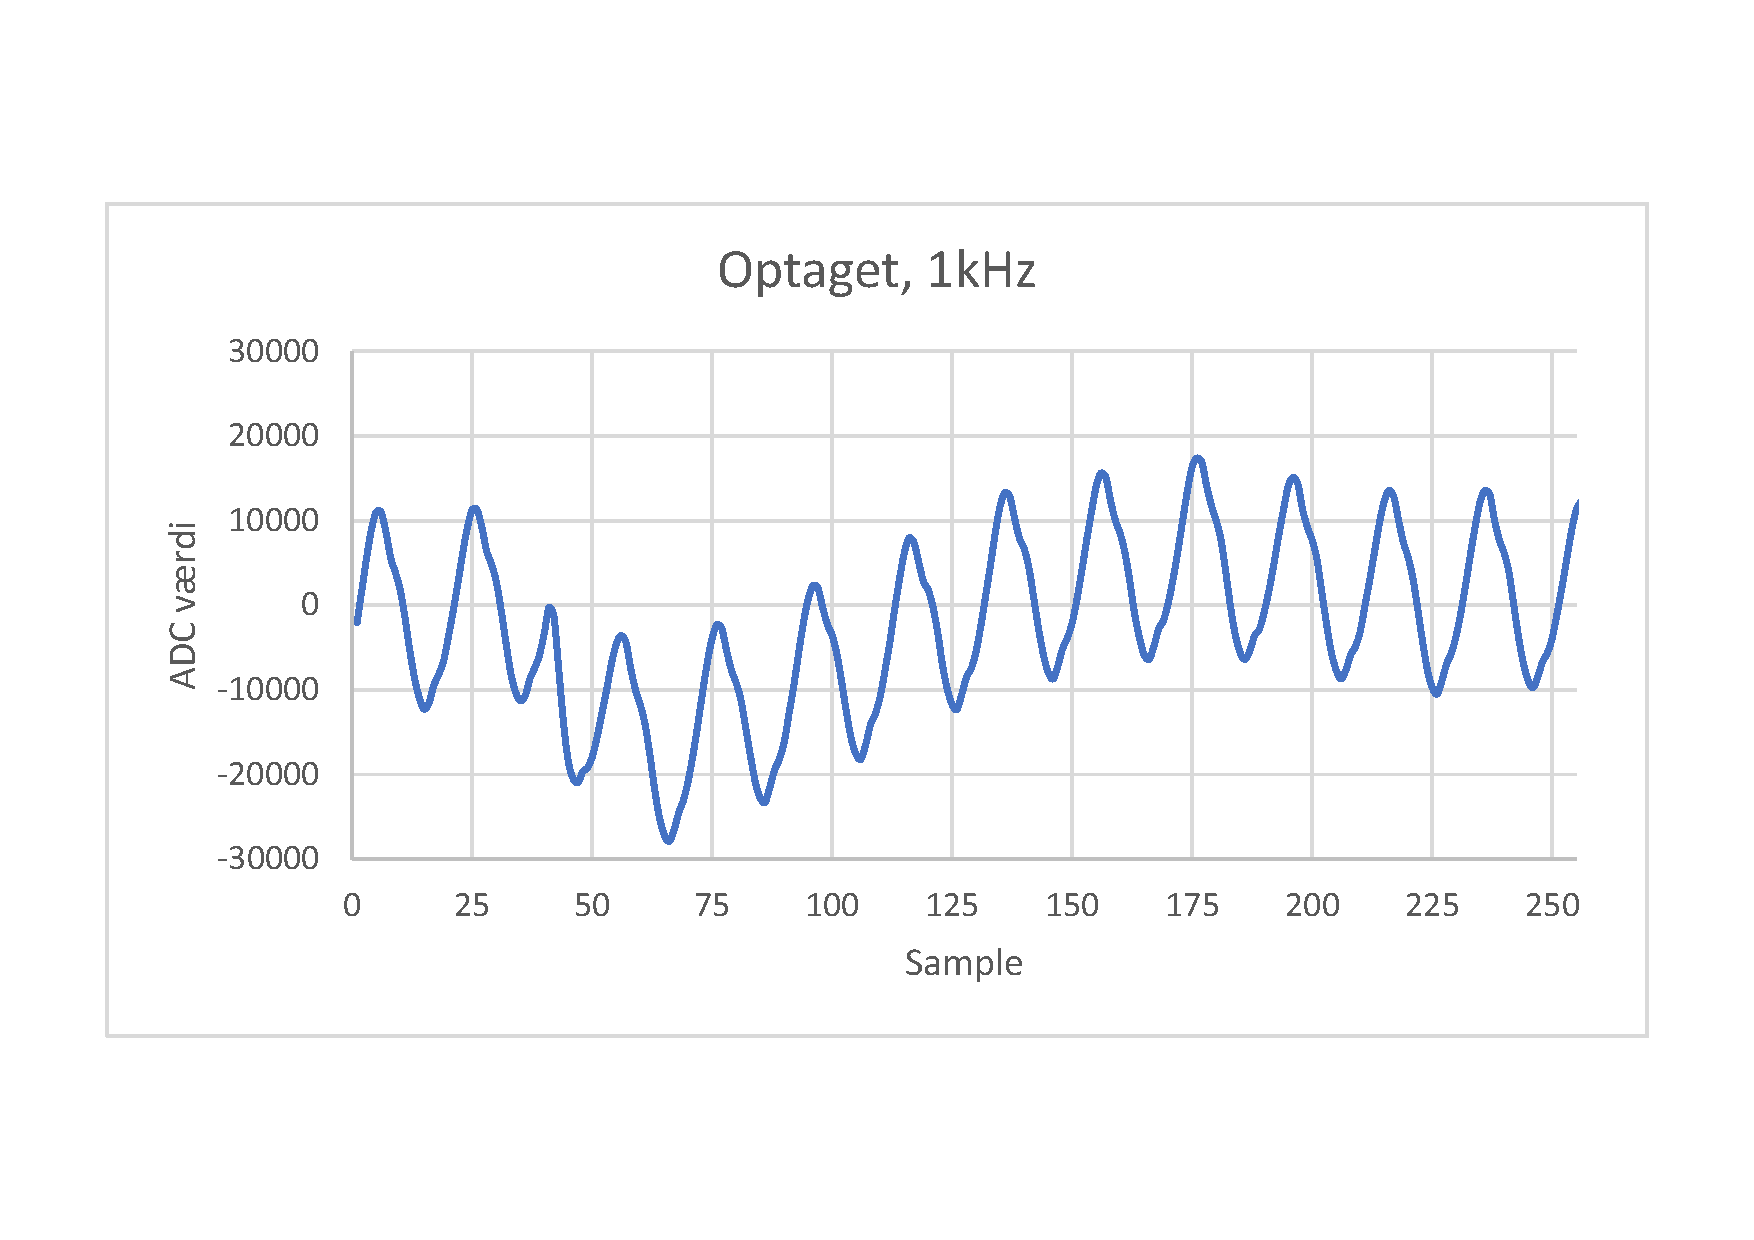
\includegraphics[width=.45\linewidth, trim={0, 2.5cm, 1.8cm, 0}, clip]{Figur/rec_time_plot.pdf}\quad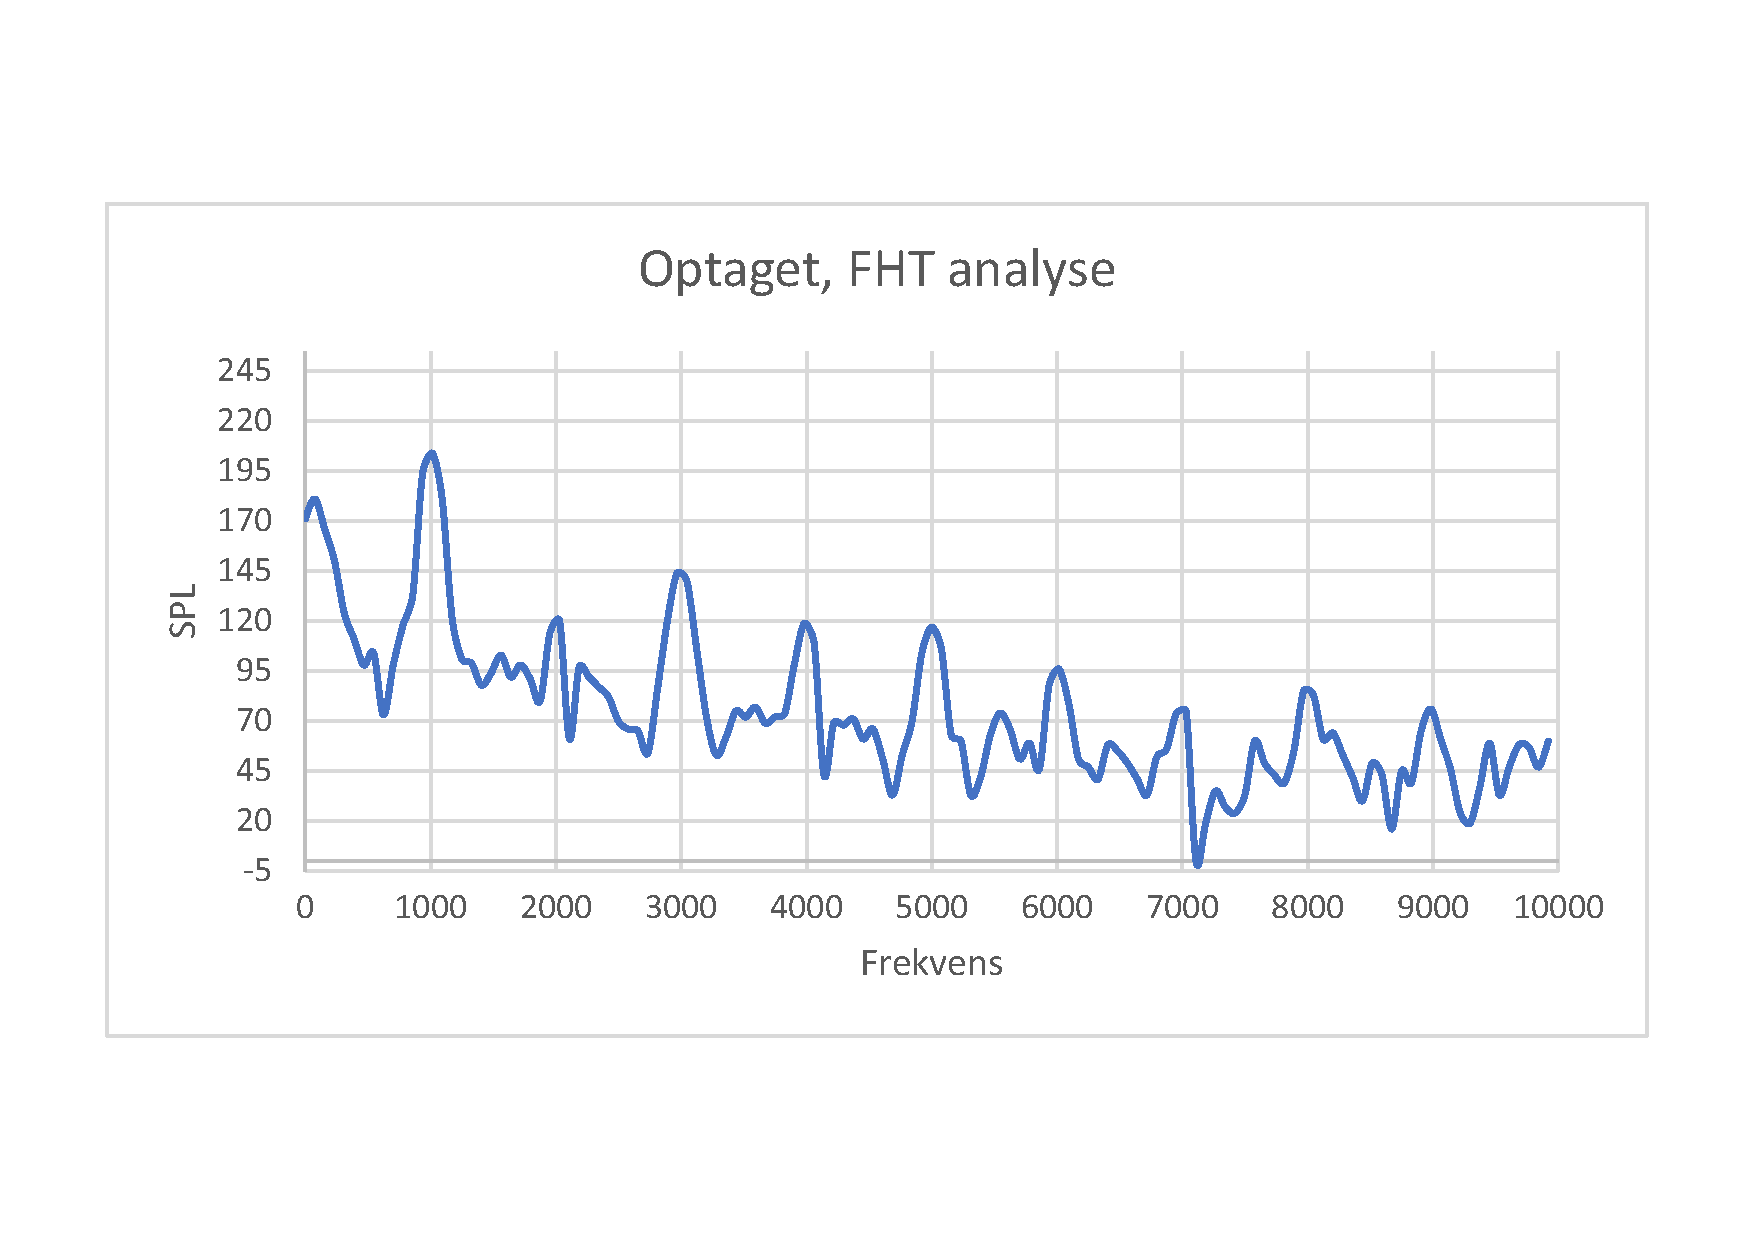
\includegraphics[width=.45\linewidth, trim={1.8cm, 2.5cm, 0cm, 0}, clip]{Figur/rec_FHT_plot}\quad
		\caption{Optagelse af 1 kHz fra mobiltelefon i tid- og frekvensdomænet }
		\label{fig:rec_plot}
	\end{center}
\end{figure}

\subsection{Modultest af skærm}
For at teste driverne til skærmen er der lavet et "dummy array" der skal simulere outputtet fra FHT modulet. Dette array lavet ved at lade et python script autogenere en c fil "DummyFHT.c". Denne fil indeholder er array (fht\_log\_out) med 128 pladser, med hver et random tal mellem 0 og 255. Disse tal repræsenterer en farve der skal vises på skærmen ved hjælp af lookup tabellen med RGB565 koderne, se figur \ref{fig:Skaerm_dummy_test}

\begin{figure} [H]
	\centering
	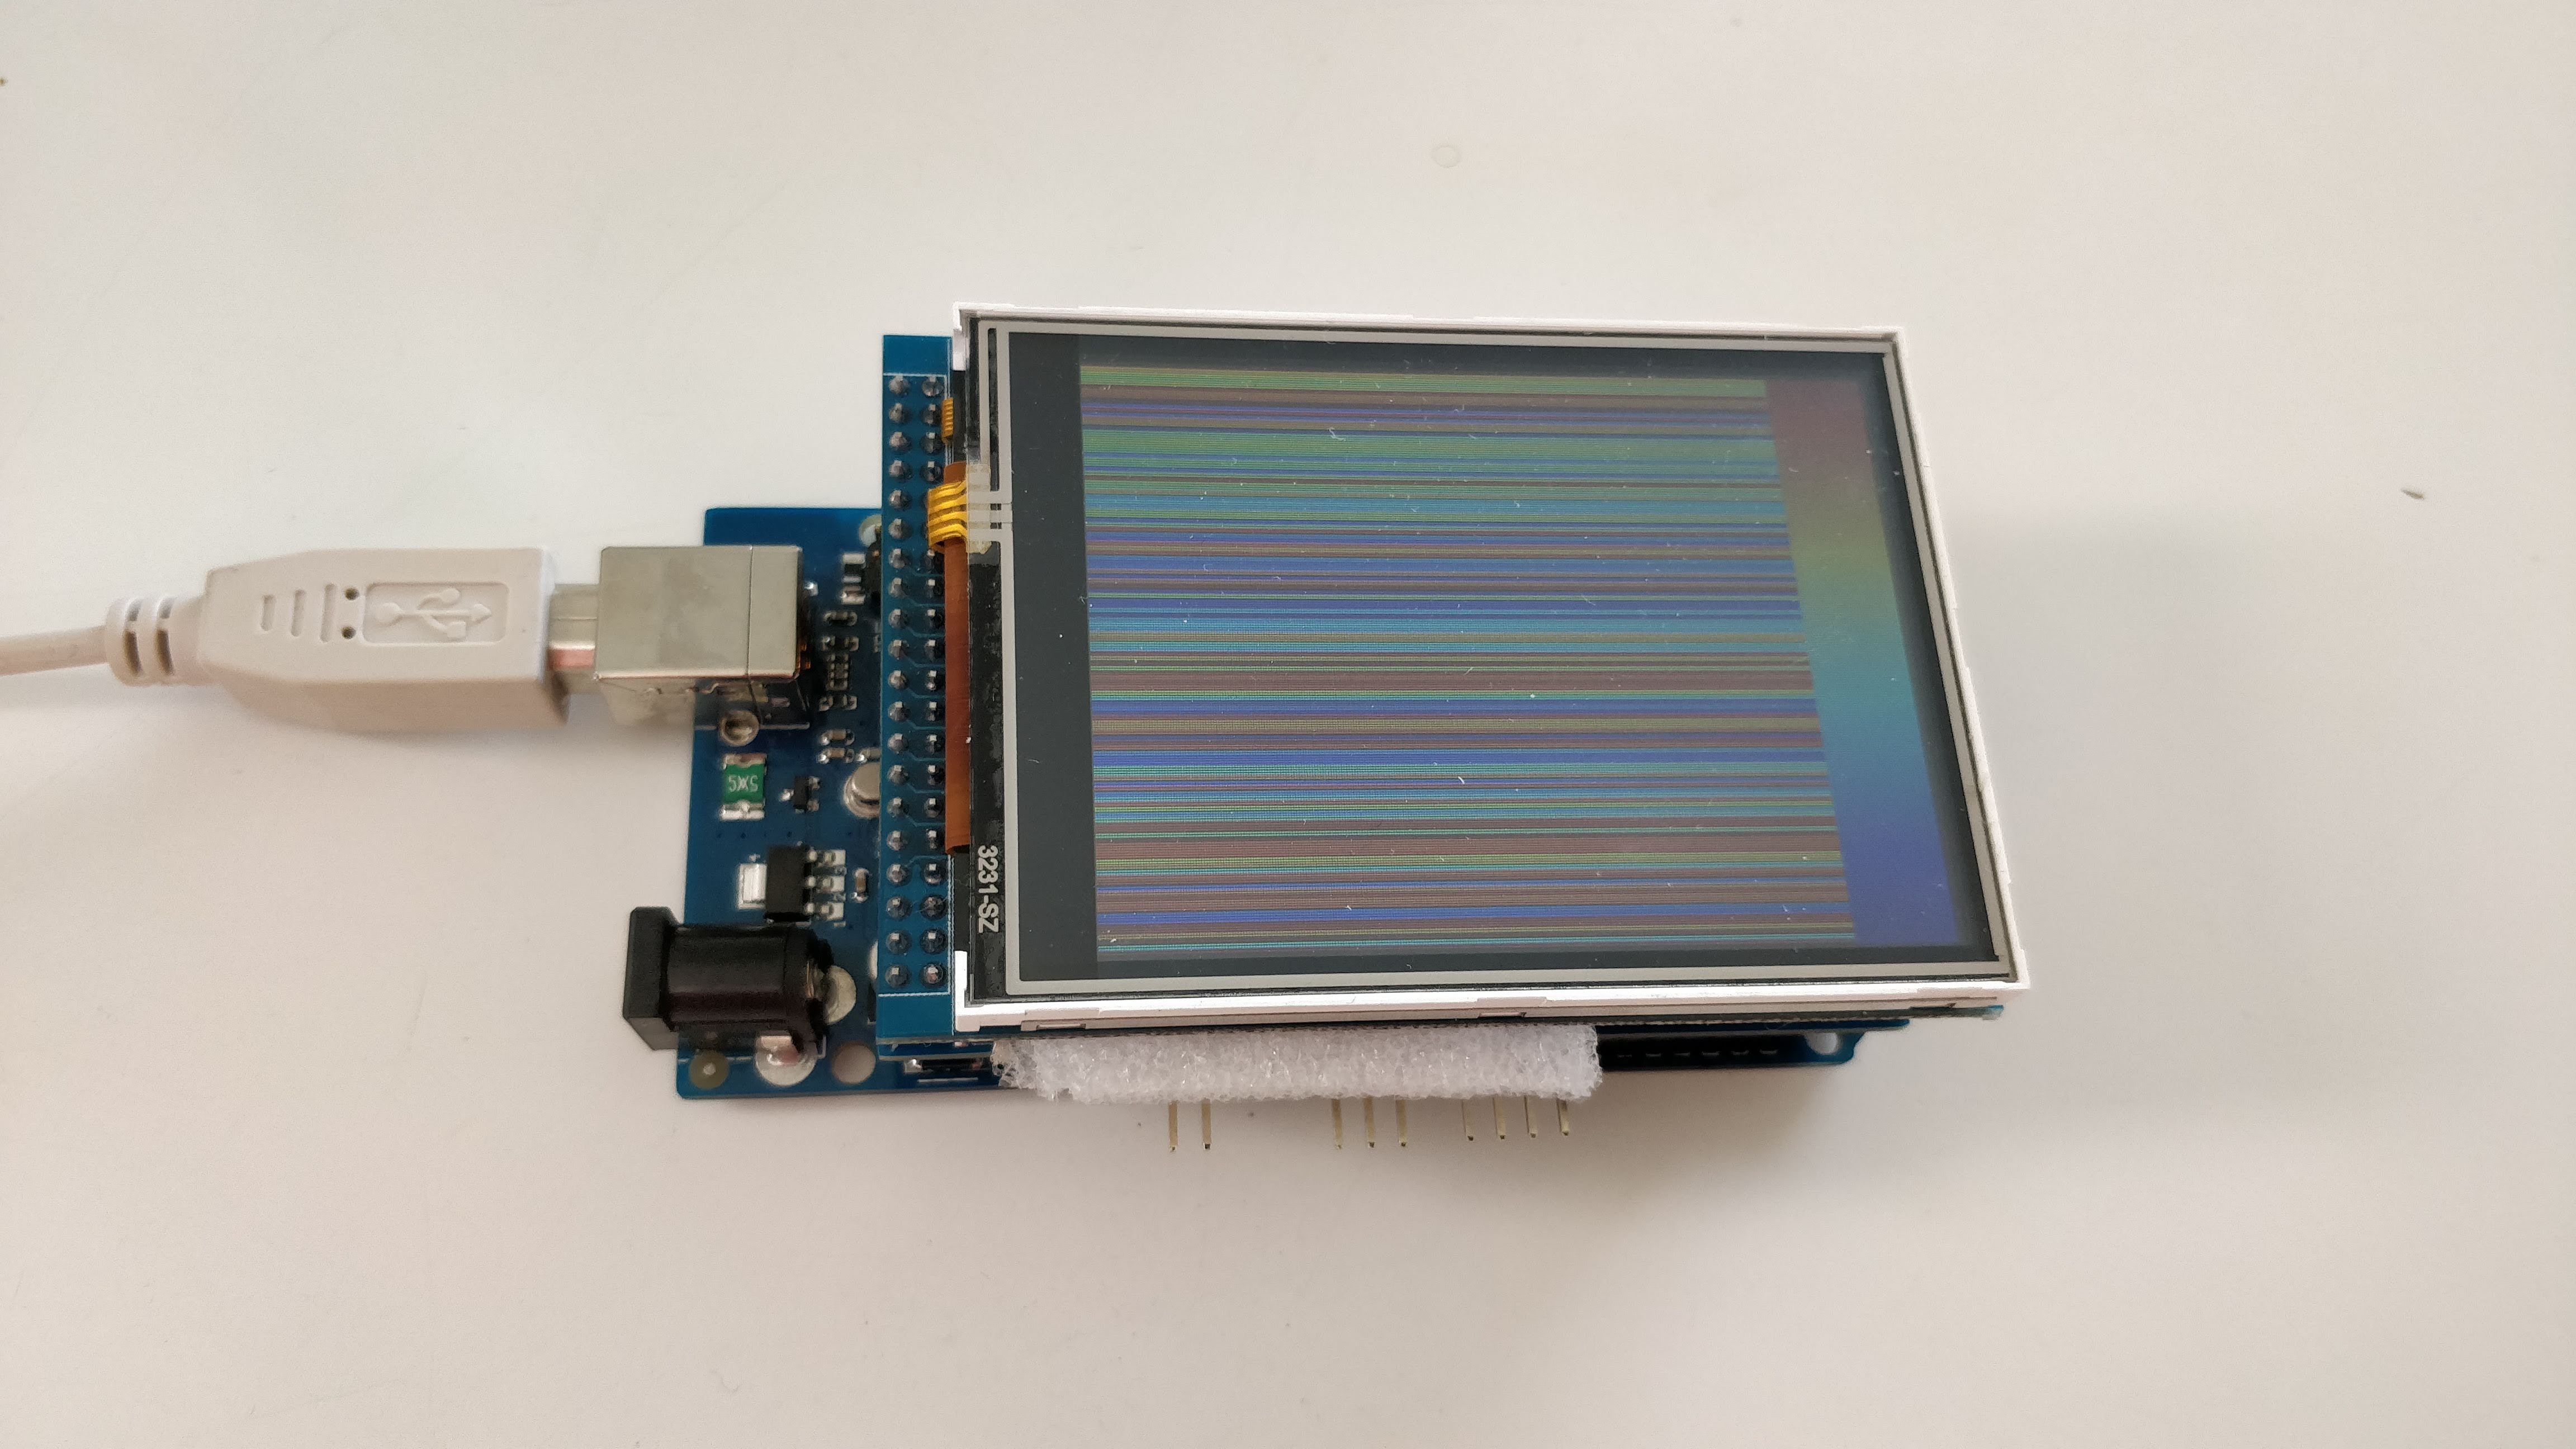
\includegraphics[width=0.7 \textwidth]{Skaerm_dummy_test.jpg}
	\captionof{figure}{Skærmtest ved hjælp af DummyFHT fil}
	\label{fig:Skaerm_dummy_test}
\end{figure}
